\documentclass{article} % For LaTeX2e
\usepackage{arxiv_template}

% Optional math commands from https://github.com/goodfeli/dlbook_notation.
% %%%%% NEW MATH DEFINITIONS %%%%%

\usepackage{amsmath,amsfonts,bm}

% Mark sections of captions for referring to divisions of figures
\newcommand{\figleft}{{\em (Left)}}
\newcommand{\figcenter}{{\em (Center)}}
\newcommand{\figright}{{\em (Right)}}
\newcommand{\figtop}{{\em (Top)}}
\newcommand{\figbottom}{{\em (Bottom)}}
\newcommand{\captiona}{{\em (a)}}
\newcommand{\captionb}{{\em (b)}}
\newcommand{\captionc}{{\em (c)}}
\newcommand{\captiond}{{\em (d)}}

% Highlight a newly defined term
\newcommand{\newterm}[1]{{\bf #1}}


% Figure reference, lower-case.
\def\figref#1{figure~\ref{#1}}
% Figure reference, capital. For start of sentence
\def\Figref#1{Figure~\ref{#1}}
\def\twofigref#1#2{figures \ref{#1} and \ref{#2}}
\def\quadfigref#1#2#3#4{figures \ref{#1}, \ref{#2}, \ref{#3} and \ref{#4}}
% Section reference, lower-case.
\def\secref#1{section~\ref{#1}}
% Section reference, capital.
\def\Secref#1{Section~\ref{#1}}
% Reference to two sections.
\def\twosecrefs#1#2{sections \ref{#1} and \ref{#2}}
% Reference to three sections.
\def\secrefs#1#2#3{sections \ref{#1}, \ref{#2} and \ref{#3}}
% Reference to an equation, lower-case.
\def\eqref#1{equation~\ref{#1}}
% Reference to an equation, upper case
\def\Eqref#1{Equation~\ref{#1}}
% A raw reference to an equation---avoid using if possible
\def\plaineqref#1{\ref{#1}}
% Reference to a chapter, lower-case.
\def\chapref#1{chapter~\ref{#1}}
% Reference to an equation, upper case.
\def\Chapref#1{Chapter~\ref{#1}}
% Reference to a range of chapters
\def\rangechapref#1#2{chapters\ref{#1}--\ref{#2}}
% Reference to an algorithm, lower-case.
\def\algref#1{algorithm~\ref{#1}}
% Reference to an algorithm, upper case.
\def\Algref#1{Algorithm~\ref{#1}}
\def\twoalgref#1#2{algorithms \ref{#1} and \ref{#2}}
\def\Twoalgref#1#2{Algorithms \ref{#1} and \ref{#2}}
% Reference to a part, lower case
\def\partref#1{part~\ref{#1}}
% Reference to a part, upper case
\def\Partref#1{Part~\ref{#1}}
\def\twopartref#1#2{parts \ref{#1} and \ref{#2}}

\def\ceil#1{\lceil #1 \rceil}
\def\floor#1{\lfloor #1 \rfloor}
\def\1{\bm{1}}
\newcommand{\train}{\mathcal{D}}
\newcommand{\valid}{\mathcal{D_{\mathrm{valid}}}}
\newcommand{\test}{\mathcal{D_{\mathrm{test}}}}

\def\eps{{\epsilon}}


% Random variables
\def\reta{{\textnormal{$\eta$}}}
\def\ra{{\textnormal{a}}}
\def\rb{{\textnormal{b}}}
\def\rc{{\textnormal{c}}}
\def\rd{{\textnormal{d}}}
\def\re{{\textnormal{e}}}
\def\rf{{\textnormal{f}}}
\def\rg{{\textnormal{g}}}
\def\rh{{\textnormal{h}}}
\def\ri{{\textnormal{i}}}
\def\rj{{\textnormal{j}}}
\def\rk{{\textnormal{k}}}
\def\rl{{\textnormal{l}}}
% rm is already a command, just don't name any random variables m
\def\rn{{\textnormal{n}}}
\def\ro{{\textnormal{o}}}
\def\rp{{\textnormal{p}}}
\def\rq{{\textnormal{q}}}
\def\rr{{\textnormal{r}}}
\def\rs{{\textnormal{s}}}
\def\rt{{\textnormal{t}}}
\def\ru{{\textnormal{u}}}
\def\rv{{\textnormal{v}}}
\def\rw{{\textnormal{w}}}
\def\rx{{\textnormal{x}}}
\def\ry{{\textnormal{y}}}
\def\rz{{\textnormal{z}}}

% Random vectors
\def\rvepsilon{{\mathbf{\epsilon}}}
\def\rvtheta{{\mathbf{\theta}}}
\def\rva{{\mathbf{a}}}
\def\rvb{{\mathbf{b}}}
\def\rvc{{\mathbf{c}}}
\def\rvd{{\mathbf{d}}}
\def\rve{{\mathbf{e}}}
\def\rvf{{\mathbf{f}}}
\def\rvg{{\mathbf{g}}}
\def\rvh{{\mathbf{h}}}
\def\rvu{{\mathbf{i}}}
\def\rvj{{\mathbf{j}}}
\def\rvk{{\mathbf{k}}}
\def\rvl{{\mathbf{l}}}
\def\rvm{{\mathbf{m}}}
\def\rvn{{\mathbf{n}}}
\def\rvo{{\mathbf{o}}}
\def\rvp{{\mathbf{p}}}
\def\rvq{{\mathbf{q}}}
\def\rvr{{\mathbf{r}}}
\def\rvs{{\mathbf{s}}}
\def\rvt{{\mathbf{t}}}
\def\rvu{{\mathbf{u}}}
\def\rvv{{\mathbf{v}}}
\def\rvw{{\mathbf{w}}}
\def\rvx{{\mathbf{x}}}
\def\rvy{{\mathbf{y}}}
\def\rvz{{\mathbf{z}}}

% Elements of random vectors
\def\erva{{\textnormal{a}}}
\def\ervb{{\textnormal{b}}}
\def\ervc{{\textnormal{c}}}
\def\ervd{{\textnormal{d}}}
\def\erve{{\textnormal{e}}}
\def\ervf{{\textnormal{f}}}
\def\ervg{{\textnormal{g}}}
\def\ervh{{\textnormal{h}}}
\def\ervi{{\textnormal{i}}}
\def\ervj{{\textnormal{j}}}
\def\ervk{{\textnormal{k}}}
\def\ervl{{\textnormal{l}}}
\def\ervm{{\textnormal{m}}}
\def\ervn{{\textnormal{n}}}
\def\ervo{{\textnormal{o}}}
\def\ervp{{\textnormal{p}}}
\def\ervq{{\textnormal{q}}}
\def\ervr{{\textnormal{r}}}
\def\ervs{{\textnormal{s}}}
\def\ervt{{\textnormal{t}}}
\def\ervu{{\textnormal{u}}}
\def\ervv{{\textnormal{v}}}
\def\ervw{{\textnormal{w}}}
\def\ervx{{\textnormal{x}}}
\def\ervy{{\textnormal{y}}}
\def\ervz{{\textnormal{z}}}

% Random matrices
\def\rmA{{\mathbf{A}}}
\def\rmB{{\mathbf{B}}}
\def\rmC{{\mathbf{C}}}
\def\rmD{{\mathbf{D}}}
\def\rmE{{\mathbf{E}}}
\def\rmF{{\mathbf{F}}}
\def\rmG{{\mathbf{G}}}
\def\rmH{{\mathbf{H}}}
\def\rmI{{\mathbf{I}}}
\def\rmJ{{\mathbf{J}}}
\def\rmK{{\mathbf{K}}}
\def\rmL{{\mathbf{L}}}
\def\rmM{{\mathbf{M}}}
\def\rmN{{\mathbf{N}}}
\def\rmO{{\mathbf{O}}}
\def\rmP{{\mathbf{P}}}
\def\rmQ{{\mathbf{Q}}}
\def\rmR{{\mathbf{R}}}
\def\rmS{{\mathbf{S}}}
\def\rmT{{\mathbf{T}}}
\def\rmU{{\mathbf{U}}}
\def\rmV{{\mathbf{V}}}
\def\rmW{{\mathbf{W}}}
\def\rmX{{\mathbf{X}}}
\def\rmY{{\mathbf{Y}}}
\def\rmZ{{\mathbf{Z}}}

% Elements of random matrices
\def\ermA{{\textnormal{A}}}
\def\ermB{{\textnormal{B}}}
\def\ermC{{\textnormal{C}}}
\def\ermD{{\textnormal{D}}}
\def\ermE{{\textnormal{E}}}
\def\ermF{{\textnormal{F}}}
\def\ermG{{\textnormal{G}}}
\def\ermH{{\textnormal{H}}}
\def\ermI{{\textnormal{I}}}
\def\ermJ{{\textnormal{J}}}
\def\ermK{{\textnormal{K}}}
\def\ermL{{\textnormal{L}}}
\def\ermM{{\textnormal{M}}}
\def\ermN{{\textnormal{N}}}
\def\ermO{{\textnormal{O}}}
\def\ermP{{\textnormal{P}}}
\def\ermQ{{\textnormal{Q}}}
\def\ermR{{\textnormal{R}}}
\def\ermS{{\textnormal{S}}}
\def\ermT{{\textnormal{T}}}
\def\ermU{{\textnormal{U}}}
\def\ermV{{\textnormal{V}}}
\def\ermW{{\textnormal{W}}}
\def\ermX{{\textnormal{X}}}
\def\ermY{{\textnormal{Y}}}
\def\ermZ{{\textnormal{Z}}}

% Vectors
\def\vzero{{\bm{0}}}
\def\vone{{\bm{1}}}
\def\vmu{{\bm{\mu}}}
\def\vtheta{{\bm{\theta}}}
\def\va{{\bm{a}}}
\def\vb{{\bm{b}}}
\def\vc{{\bm{c}}}
\def\vd{{\bm{d}}}
\def\ve{{\bm{e}}}
\def\vf{{\bm{f}}}
\def\vg{{\bm{g}}}
\def\vh{{\bm{h}}}
\def\vi{{\bm{i}}}
\def\vj{{\bm{j}}}
\def\vk{{\bm{k}}}
\def\vl{{\bm{l}}}
\def\vm{{\bm{m}}}
\def\vn{{\bm{n}}}
\def\vo{{\bm{o}}}
\def\vp{{\bm{p}}}
\def\vq{{\bm{q}}}
\def\vr{{\bm{r}}}
\def\vs{{\bm{s}}}
\def\vt{{\bm{t}}}
\def\vu{{\bm{u}}}
\def\vv{{\bm{v}}}
\def\vw{{\bm{w}}}
\def\vx{{\bm{x}}}
\def\vy{{\bm{y}}}
\def\vz{{\bm{z}}}

% Elements of vectors
\def\evalpha{{\alpha}}
\def\evbeta{{\beta}}
\def\evepsilon{{\epsilon}}
\def\evlambda{{\lambda}}
\def\evomega{{\omega}}
\def\evmu{{\mu}}
\def\evpsi{{\psi}}
\def\evsigma{{\sigma}}
\def\evtheta{{\theta}}
\def\eva{{a}}
\def\evb{{b}}
\def\evc{{c}}
\def\evd{{d}}
\def\eve{{e}}
\def\evf{{f}}
\def\evg{{g}}
\def\evh{{h}}
\def\evi{{i}}
\def\evj{{j}}
\def\evk{{k}}
\def\evl{{l}}
\def\evm{{m}}
\def\evn{{n}}
\def\evo{{o}}
\def\evp{{p}}
\def\evq{{q}}
\def\evr{{r}}
\def\evs{{s}}
\def\evt{{t}}
\def\evu{{u}}
\def\evv{{v}}
\def\evw{{w}}
\def\evx{{x}}
\def\evy{{y}}
\def\evz{{z}}

% Matrix
\def\mA{{\bm{A}}}
\def\mB{{\bm{B}}}
\def\mC{{\bm{C}}}
\def\mD{{\bm{D}}}
\def\mE{{\bm{E}}}
\def\mF{{\bm{F}}}
\def\mG{{\bm{G}}}
\def\mH{{\bm{H}}}
\def\mI{{\bm{I}}}
\def\mJ{{\bm{J}}}
\def\mK{{\bm{K}}}
\def\mL{{\bm{L}}}
\def\mM{{\bm{M}}}
\def\mN{{\bm{N}}}
\def\mO{{\bm{O}}}
\def\mP{{\bm{P}}}
\def\mQ{{\bm{Q}}}
\def\mR{{\bm{R}}}
\def\mS{{\bm{S}}}
\def\mT{{\bm{T}}}
\def\mU{{\bm{U}}}
\def\mV{{\bm{V}}}
\def\mW{{\bm{W}}}
\def\mX{{\bm{X}}}
\def\mY{{\bm{Y}}}
\def\mZ{{\bm{Z}}}
\def\mBeta{{\bm{\beta}}}
\def\mPhi{{\bm{\Phi}}}
\def\mLambda{{\bm{\Lambda}}}
\def\mSigma{{\bm{\Sigma}}}

% Tensor
\DeclareMathAlphabet{\mathsfit}{\encodingdefault}{\sfdefault}{m}{sl}
\SetMathAlphabet{\mathsfit}{bold}{\encodingdefault}{\sfdefault}{bx}{n}
\newcommand{\tens}[1]{\bm{\mathsfit{#1}}}
\def\tA{{\tens{A}}}
\def\tB{{\tens{B}}}
\def\tC{{\tens{C}}}
\def\tD{{\tens{D}}}
\def\tE{{\tens{E}}}
\def\tF{{\tens{F}}}
\def\tG{{\tens{G}}}
\def\tH{{\tens{H}}}
\def\tI{{\tens{I}}}
\def\tJ{{\tens{J}}}
\def\tK{{\tens{K}}}
\def\tL{{\tens{L}}}
\def\tM{{\tens{M}}}
\def\tN{{\tens{N}}}
\def\tO{{\tens{O}}}
\def\tP{{\tens{P}}}
\def\tQ{{\tens{Q}}}
\def\tR{{\tens{R}}}
\def\tS{{\tens{S}}}
\def\tT{{\tens{T}}}
\def\tU{{\tens{U}}}
\def\tV{{\tens{V}}}
\def\tW{{\tens{W}}}
\def\tX{{\tens{X}}}
\def\tY{{\tens{Y}}}
\def\tZ{{\tens{Z}}}


% Graph
\def\gA{{\mathcal{A}}}
\def\gB{{\mathcal{B}}}
\def\gC{{\mathcal{C}}}
\def\gD{{\mathcal{D}}}
\def\gE{{\mathcal{E}}}
\def\gF{{\mathcal{F}}}
\def\gG{{\mathcal{G}}}
\def\gH{{\mathcal{H}}}
\def\gI{{\mathcal{I}}}
\def\gJ{{\mathcal{J}}}
\def\gK{{\mathcal{K}}}
\def\gL{{\mathcal{L}}}
\def\gM{{\mathcal{M}}}
\def\gN{{\mathcal{N}}}
\def\gO{{\mathcal{O}}}
\def\gP{{\mathcal{P}}}
\def\gQ{{\mathcal{Q}}}
\def\gR{{\mathcal{R}}}
\def\gS{{\mathcal{S}}}
\def\gT{{\mathcal{T}}}
\def\gU{{\mathcal{U}}}
\def\gV{{\mathcal{V}}}
\def\gW{{\mathcal{W}}}
\def\gX{{\mathcal{X}}}
\def\gY{{\mathcal{Y}}}
\def\gZ{{\mathcal{Z}}}

% Sets
\def\sA{{\mathbb{A}}}
\def\sB{{\mathbb{B}}}
\def\sC{{\mathbb{C}}}
\def\sD{{\mathbb{D}}}
% Don't use a set called E, because this would be the same as our symbol
% for expectation.
\def\sF{{\mathbb{F}}}
\def\sG{{\mathbb{G}}}
\def\sH{{\mathbb{H}}}
\def\sI{{\mathbb{I}}}
\def\sJ{{\mathbb{J}}}
\def\sK{{\mathbb{K}}}
\def\sL{{\mathbb{L}}}
\def\sM{{\mathbb{M}}}
\def\sN{{\mathbb{N}}}
\def\sO{{\mathbb{O}}}
\def\sP{{\mathbb{P}}}
\def\sQ{{\mathbb{Q}}}
\def\sR{{\mathbb{R}}}
\def\sS{{\mathbb{S}}}
\def\sT{{\mathbb{T}}}
\def\sU{{\mathbb{U}}}
\def\sV{{\mathbb{V}}}
\def\sW{{\mathbb{W}}}
\def\sX{{\mathbb{X}}}
\def\sY{{\mathbb{Y}}}
\def\sZ{{\mathbb{Z}}}

% Entries of a matrix
\def\emLambda{{\Lambda}}
\def\emA{{A}}
\def\emB{{B}}
\def\emC{{C}}
\def\emD{{D}}
\def\emE{{E}}
\def\emF{{F}}
\def\emG{{G}}
\def\emH{{H}}
\def\emI{{I}}
\def\emJ{{J}}
\def\emK{{K}}
\def\emL{{L}}
\def\emM{{M}}
\def\emN{{N}}
\def\emO{{O}}
\def\emP{{P}}
\def\emQ{{Q}}
\def\emR{{R}}
\def\emS{{S}}
\def\emT{{T}}
\def\emU{{U}}
\def\emV{{V}}
\def\emW{{W}}
\def\emX{{X}}
\def\emY{{Y}}
\def\emZ{{Z}}
\def\emSigma{{\Sigma}}

% entries of a tensor
% Same font as tensor, without \bm wrapper
\newcommand{\etens}[1]{\mathsfit{#1}}
\def\etLambda{{\etens{\Lambda}}}
\def\etA{{\etens{A}}}
\def\etB{{\etens{B}}}
\def\etC{{\etens{C}}}
\def\etD{{\etens{D}}}
\def\etE{{\etens{E}}}
\def\etF{{\etens{F}}}
\def\etG{{\etens{G}}}
\def\etH{{\etens{H}}}
\def\etI{{\etens{I}}}
\def\etJ{{\etens{J}}}
\def\etK{{\etens{K}}}
\def\etL{{\etens{L}}}
\def\etM{{\etens{M}}}
\def\etN{{\etens{N}}}
\def\etO{{\etens{O}}}
\def\etP{{\etens{P}}}
\def\etQ{{\etens{Q}}}
\def\etR{{\etens{R}}}
\def\etS{{\etens{S}}}
\def\etT{{\etens{T}}}
\def\etU{{\etens{U}}}
\def\etV{{\etens{V}}}
\def\etW{{\etens{W}}}
\def\etX{{\etens{X}}}
\def\etY{{\etens{Y}}}
\def\etZ{{\etens{Z}}}

% The true underlying data generating distribution
\newcommand{\pdata}{p_{\rm{data}}}
% The empirical distribution defined by the training set
\newcommand{\ptrain}{\hat{p}_{\rm{data}}}
\newcommand{\Ptrain}{\hat{P}_{\rm{data}}}
% The model distribution
\newcommand{\pmodel}{p_{\rm{model}}}
\newcommand{\Pmodel}{P_{\rm{model}}}
\newcommand{\ptildemodel}{\tilde{p}_{\rm{model}}}
% Stochastic autoencoder distributions
\newcommand{\pencode}{p_{\rm{encoder}}}
\newcommand{\pdecode}{p_{\rm{decoder}}}
\newcommand{\precons}{p_{\rm{reconstruct}}}

\newcommand{\laplace}{\mathrm{Laplace}} % Laplace distribution

\newcommand{\E}{\mathbb{E}}
\newcommand{\Ls}{\mathcal{L}}
\newcommand{\R}{\mathbb{R}}
\newcommand{\emp}{\tilde{p}}
\newcommand{\lr}{\alpha}
\newcommand{\reg}{\lambda}
\newcommand{\rect}{\mathrm{rectifier}}
\newcommand{\softmax}{\mathrm{softmax}}
\newcommand{\sigmoid}{\sigma}
\newcommand{\softplus}{\zeta}
\newcommand{\KL}{D_{\mathrm{KL}}}
\newcommand{\Var}{\mathrm{Var}}
\newcommand{\standarderror}{\mathrm{SE}}
\newcommand{\Cov}{\mathrm{Cov}}
% Wolfram Mathworld says $L^2$ is for function spaces and $\ell^2$ is for vectors
% But then they seem to use $L^2$ for vectors throughout the site, and so does
% wikipedia.
\newcommand{\normlzero}{L^0}
\newcommand{\normlone}{L^1}
\newcommand{\normltwo}{L^2}
\newcommand{\normlp}{L^p}
\newcommand{\normmax}{L^\infty}

\newcommand{\parents}{Pa} % See usage in notation.tex. Chosen to match Daphne's book.

\DeclareMathOperator*{\argmax}{arg\,max}
\DeclareMathOperator*{\argmin}{arg\,min}

\DeclareMathOperator{\sign}{sign}
\DeclareMathOperator{\Tr}{Tr}
\let\ab\allowbreak


\usepackage{microtype}
\usepackage{hyperref}
\usepackage{url}
\usepackage{graphicx}

\usepackage{pgfplots}
\usepackage{pgfplotstable}
\pgfplotsset{compat=1.3}
\usepackage{tikz}
\usetikzlibrary{arrows.meta}
\usetikzlibrary{pgfplots.groupplots}
\usepackage{ragged2e}
\definecolor{mydarkblue}{rgb}{0,0.08,0.85}
\definecolor{mylightblue}{rgb}{0.06,0.56,1.0}
\definecolor{mylightorange}{rgb}{1.0,0.62,0.12}
\definecolor{mylightred}{rgb}{0.99,0.00,0.04}
\definecolor{mygreen}{HTML}{2F9E44}
\definecolor{myred}{HTML}{E03131}
\definecolor{myblue}{HTML}{1971C2}

\usepackage{subcaption}
\usepackage{booktabs}
\usepackage{wrapfig}
\usepackage{changes}
\definecolor{myred}{HTML}{E03131}
\makeatletter
\@namedef{Changes@AuthorColor}{myred}
\colorlet{Changes@Color}{myred}
\makeatother
% \usepackage{floatrow}
\colmfinalcopy

% \def\l{\left}
% \def\r{\right}

\title{\texttt{mandala}: Compositional Memoization for Simple \&
Powerful Scientific Data Management}

\newcommand{\fix}{\marginpar{FIX}}
\newcommand{\new}{\marginpar{NEW}}
% \newfloatcommand{capbtabbox}{table}[][\FBwidth]

\usepackage{soul}
\usepackage{amsthm}
\usepackage{mathrsfs}
% \usepackage[outputdir=/home/amakelov/vscode_output/latex-aux]{minted}
\newtheorem{theorem}{Theorem}[section]
\newtheorem{lemma}[theorem]{Lemma}



\begin{document}
\maketitle


\begin{abstract}
  We present
  \texttt{mandala}\footnote{\url{https://github.com/amakelov/mandala}}, a Python
  library that largely eliminates the accidental complexity of scientific data
  management and incremental computing. While most traditional and/or
  popular data management solutions are based on \emph{logging},
  \texttt{mandala} takes a fundamentally different approach, using
  \emph{memoization} of function calls as the fundamental unit of saving,
  loading, querying and deleting computational artifacts. 
  
  It does so by implementing a \emph{compositional} form of memoization, which keeps
  track of how memoized functions compose with one another. In this way: (1)
  complex computations are effectively memoized end-to-end, and become
  `interfaces' to their own intermediate results by retracing the memoized
  calls; (2) all computations in a project form a single computational graph,
  which can be explored, queried and manipulated in high-level ways through a
  \emph{computation frame}, which is a natural generalization of a dataframe that replaces columns by a computation graph, and rows by (partial) executions of this graph.

  Several features implemented on top of the core memoization data structures ---
  such as natively and transparently handling Python collections, in-memory caching of
  intermediate results, and a flexible versioning system with dynamic dependency
  tracking --- turn \texttt{mandala} into a practical and simple tool for
  managing and interacting with computational data.
\end{abstract}

\section{Introduction}
\label{section:intro}

Numerical experiments and simulations are growing into a central part of many
areas of science and engineering \citep{hey2009fourth}. Recent trends in
computation-intensive fields, such as machine learning, point towards (1)
ever-increasing complexity of computational pipelines, and (2) adoption in more
safety-critical domains, such as autonomous driving \citep{bojarski2016end} and
healthcare \citep{ravi2016deep,abramson2024accurate}.

These developments impose opposing constraints on the tools used to manage the
resulting computational artifacts. On the one hand, they should be simple and
easy to use by researchers, with a minimal learning curve and unobtrusive syntax
and semantics. On the other hand, they should deliver a lot of added
functionality, such as high-level operations \citep{wickham2014tidy}, full data
\& code provenance auditing \citep{davidson2008provenance} and reproducibility
\citep{ivie2018reproducibility} in complex projects.  Rules and best practices
that help with these requirements exist and are well-known
\citep{sandve2013ten,wilkinson2016fair}, but still require manual effort,
attention to extraneous details, and discipline to follow. Researchers often
operate under time pressure and/or the need to quickly iterate on code, which
makes these best `practices' a rather \emph{impractical} time investment. 

Thus, ideally we would like a system that (1) does not get in the way by
imposing a complex new language/semantics/syntax, (2) provides powerful
high-level data management operations over complex computational projects, and
(3) incorporates best practices by design and without cognitive overhead.

% a figure with 3 subfigures side by side, each with a caption. Each figure is an imported .pdf file
\begin{figure}[h]
\centering
\begin{subfigure}{0.23\textwidth}
\centering
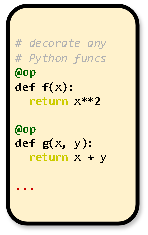
\includegraphics[width=\textwidth]{img/fig1.pdf}
\caption{}
\end{subfigure}
\begin{subfigure}{0.35\textwidth}
\centering
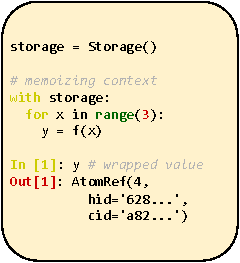
\includegraphics[width=\textwidth]{img/fig2.pdf}
\caption{}
\end{subfigure}
\begin{subfigure}{0.4\textwidth}
\centering
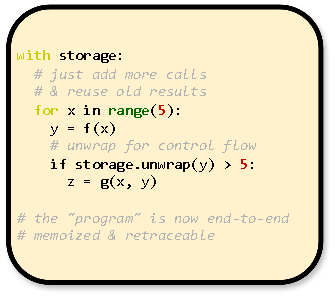
\includegraphics[width=\textwidth]{img/fig3.pdf}
\caption{}
\end{subfigure}
\caption{Basic imperative usage of \texttt{mandala}. \textbf{(a)}: add the \texttt{@op}
decorator to any Python functions to make them memoizable. \textbf{(b)}:
create a \texttt{Storage}, and use it as a context manager to automatically
memoize any calls to \texttt{@op}-decorated functions in the block. Memoized
functions return \texttt{Ref} objects, which wrap a value with two pieces of
metadata: a \emph{content ID}, which is a hash of the value of the
object, and a \emph{history ID}, which is a hash of the identity of the
\texttt{@op} that produced the \texttt{Ref} (if any), and the history IDs of the
\texttt{@op}'s inputs. \textbf{(c)}: the storage context allows simple
incremental computation and recovery from failures. Here, we add more
computations while automatically reusing already computed values.}
\label{fig:basic-usage}
\end{figure}

In this paper we present \texttt{mandala}, our proposal for such a system. It \textbf{integrates data management logic and best practices} such as
\begin{itemize}
\item Full data provenance tracking
\item Idempotent \& reproducible computation
\item Content-addressable versioning of code and its dependencies
\item Declarative high-level manipulation of persisted computational graphs
\end{itemize}
\textbf{into Python's already familiar syntax and semantics} (Figures
\ref{fig:basic-usage} and \ref{fig:cf}). The integration aims to be maximally
transparent and unobtrusive, so that the user can focus on the \emph{essential
complexity} (the scientific problem at hand), rather than on the
\emph{accidental complexity} (the data management tools necessary to implement the solution) \citep{Brooks1987NoSB}.

The rest of this paper presents the design and main functionalities of
\texttt{mandala}, and is organized as follows: 
\begin{itemize}
\item In Section \ref{section:core-concepts}, we describe how memoization is
designed, how this allows memoized calls to be composed and memoized results to
be reused without storage duplication, and how this enables the \emph{retracing}
pattern of interacting with computational artifacts.
\item In Section \ref{section:cf}, we introduce the concept of a
\emph{computation frame}, which generalizes a dataframe by replacing columns
with a computational graph, and rows with individual computations that
(partially) follow this graph. Computation frames allow high-level exploration
and manipulation of the stored computation graph, such as adding the calls that
produced/used given values to the graph, deleting all computations that depend
on the calls captured in the frame, and restricting the frame to a particular
subgraph or subset of values with given properties.
\item In Section \ref{section:extra-features}, we describe some other features of
\texttt{mandala} necessary to make it a practical tool, such as:
\begin{itemize}
\item Representing Python collections in a way transparent to the storage, so
that the membership relationships between a collection and its items are
propagated through the saved computational graph;
\item Caching of intermediate results to speed up retracing and memoization;
\item A flexible versioning system with automatic dynamic dependency tracking.
\end{itemize}
\end{itemize}

Finally, we give an overview of related work in Section \ref{section:related-work}.

\section{Core Concepts}
\label{section:core-concepts}

\subsection{Memoization and the Computational Graph}

Memoization is a technique that stores the results of expensive function calls
to avoid redundant computation. \texttt{mandala} uses \emph{automatic}
memoization \citep{norvig1991techniques} which is applied via the combination of
a decorator (\texttt{@op}) and a context manager which specifies the
\texttt{Storage} object to use (Figure \ref{fig:basic-usage}). The memoization
can optionally be made persistent to disk, which is what you would typically
want in a long-running project. Any Python function can be memoized (as long as
its inputs and outputs are serializable by the \texttt{joblib} library; see the
limitations section \ref{sec:limitations} for caveats); there is no restriction
on the type, number or naming scheme (positional, keyword, variadic, or variable
keyword) of the arguments or return values.

\paragraph{\texttt{Call} and \texttt{Ref} objects, and content/history IDs.}
\texttt{Ref}s and \texttt{Call}s are the two atomic data structures in
\texttt{mandala}'s model of computations. When a call to an
\texttt{@op}-decorated function \texttt{f} is executed inside a storage context,
this results in the creation of 
\begin{itemize}
\item A \texttt{Ref} object for each input to the call. These wrap the `raw'
values passed as inputs together with content IDs (hashes of the Python objects)
and history IDs (hashes of the memoized calls that produced these values, if
any). 
\begin{itemize}
\item If an input to the call is already a \texttt{Ref} object, it is passed
through as is;
\item If it is a `raw' (i.e., non-\texttt{Ref}) value, a new \texttt{Ref} object
is created with a `empty' history ID that is simply a hash of the content ID
itself.
\end{itemize}
\item A \texttt{Call} object, which has pointers to the input and output
(defined below) \texttt{Ref}s of the call to \texttt{f}, as well as a content ID
for the call (a hash of the identity of \texttt{f} and the content IDs of the
input \texttt{Ref}s) and a history ID (by analogy, a hash of the identity of
\texttt{f} and the history IDs of the inputs). The version of \texttt{f} is also part of the identity of \texttt{f}; see the versioning section \ref{subsection:versioning} for details.
\item A \texttt{Ref} object for each return value of the call. These are again
assigned content IDs by value, and history IDs by hashing the tuple (history ID
of the call, corresponding output name\footnote{Since Python functions don't
have designated output names, we instead generate output names automatically using the order in the tuple of return values.}).
\end{itemize}

% \begin{wrapfigure}[18]{r}{0.5\textwidth}
%     \centering
%     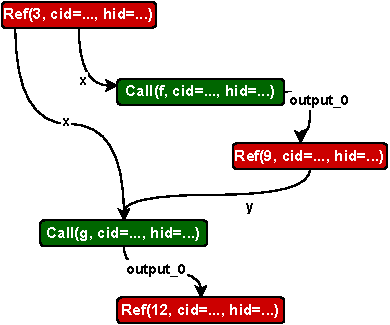
\includegraphics[width=\linewidth]{img/comp-graph.pdf}
%     \caption{A part of the computaitonal graph built up by the calls in Figure
%     \ref{fig:basic-usage}. 
%     % The nodes are \texttt{Call} and \texttt{Ref} objects,
%     % and the edges are the inputs/output names connecting them.
%     }
%     \label{fig:comp-graph}
% \end{wrapfigure}


The \texttt{Ref}s and the \texttt{Call} are then stored in the storage backend,
and the next time \texttt{f} is called on inputs that have the same
\emph{content} IDs, the stored \texttt{Call} is looked up to find the output
\texttt{Ref}s, which are then returned (possibly with properly updated history
IDs, if the call exists in storage by content ID only). The combination of all
stored \texttt{Call}s and \texttt{Ref}s across memoized functions form the
\textbf{computational graph} represented by the storage. Importantly, the
`interesting' structure of this graph is built up automatically by the way the
user composes memoized calls.

\subsection{Motivation for the Design of Memoization}
\label{subsection:}

\paragraph{Why content and history IDs?}
The simultaneous use of content and history IDs has a few subtle advantages.
First, it allows for the \emph{de-duplication} of storage, as the same content
ID can be used to store the same value produced by different computations. For
instance, there may be many computaitions all producing the value $42$ (or a
large all-zero array), but only one copy of $42$ is stored in the backend. At
the same time, the history IDs allow us to distinguish between computations that
produced the same value, but in different ways. This avoids `parasitic' results
in declarative queries. For example, a call to \texttt{f} may result in 42, and
we may be interested in all calls that were ran on this particular 42 returned
by \texttt{f} and not on any other \texttt{Ref} whose value happens to be 42.
Without history IDs, it would be impossible to make this distinction in the
stored computational graph.


\paragraph{Why memoization?} Memoization is an unusual choice for data
management systems, most of which are based on \emph{logging}, i.e. explicitly
pointing to the value to be saved and the address where it should be saved
(whether this is some kind of name or a file path). Basing data management on
memoization means that the `address' of a value is now implicit in the code that
produced it, and the value itself is stored in a shared storage backend. This has several advantages:
\begin{itemize}
\item It \textbf{eliminates the need to manually name artifacts}. This
eliminates a major source of accidental complexity: names are arbitrary,
ambiguous, and can drift away from the actual content of the value they point to
over time. On the other hand, names are not strictly necessary, because the
composition of memoized functions that produced a given value --- which must be
specified anyway for the computation to take place --- is already an unambiguous
pointer to it.
\item Since the \texttt{@op} decorator encourages (and in a sense enforces)
composition of \texttt{@op}s, it \textbf{automatically builds up a computational
graph of the project}. Most data management tasks --- e.g., a frequent use case
is getting a table of relationships between some variables --- are naturally
expressed as queries over this graph, as we will see in Section
\ref{section:cf}.
\item It \textbf{organizes storage functionality around a familiar and flexible
interface: the function call}. This automatically enforces the good practice
of partitioning code into functions, and eliminates extra `accidental' code to
save and load values explicitly. Furthermore, it synchronizes failures between
computation and storage, as the memoized calls are the natural points to
recover from.
\end{itemize}

On the other hand, memoization suffers from the following limitations:
\begin{itemize}
\item Referring to values without reference to the code that produced or used
them becomes difficult, because from the point of view of storage the `identity'
of a value is its place in the computational graph. We discuss practical ways to
overcome this in Section \ref{section:cf}.
\item Modifying \texttt{@op} functions requires care, as changes may invalidate
the stored computational graph. We discuss a versioning system that automates this process in Section \ref{subsection:versioning}.
\end{itemize}

\subsection{Retracing as a Versatile Imperative Interface to the Stored Computation Graph}
\label{subsection:retracing}

The compositional nature of memoization makes it possible to build complex
computations out of calls to memoized functions, turning the entire computation
into an end-to-end-memoized interface to its own intermediate results. The main
way to interact with such a persisted computation is through \textbf{retracing},
which means stepping through memoized code with the purpose of resuming from a
failure, loading intermediate values, or continuing from a particular point with
new computations. A small example of retracing is shown in Figure
\ref{fig:basic-usage} (c). 

This pattern is simple yet powerful, as it allows the user to interact with the
stored computation graph in a way that is adapted to their use case, and to
explore the graph in a way that is natural and familiar to them. It also
simplifies the management of state in an interactive environment such as a
Jupyter notebook, because it makes it very cheap to re-run cells in order to recreate the intended state of local variables.

\section{Computation Frames}
\label{section:cf}

\begin{figure}[htbp]
    \centering
    \begin{minipage}[b]{0.48\textwidth}
        \begin{subfigure}[b]{\textwidth}
            \centering
            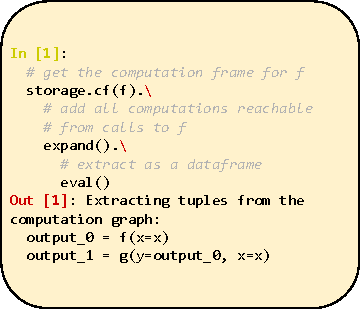
\includegraphics[width=\textwidth]{img/fig4.pdf}
            \caption{Continuing from Figure \ref{fig:basic-usage}, we first
            create a computation frame from a single function \texttt{f}, then
            expand it to include all calls that can be reached from the memoized
            calls to \texttt{f} via their inputs/outputs, and finally convert
            the computation frame into a dataframe. We see that this
            automatically produces a computation graph corresponding to the
            computations found.}
            \label{fig:figure1}
        \end{subfigure}
        
        \vspace{1em}
        
        \begin{subfigure}[b]{\textwidth}
            \centering
            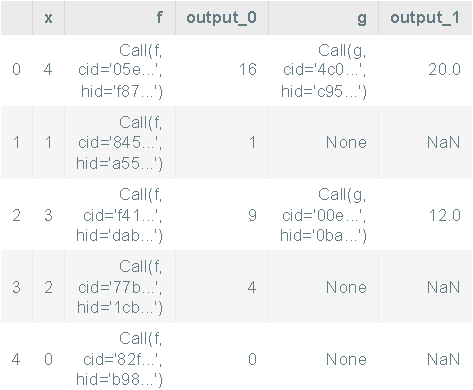
\includegraphics[width=\textwidth]{img/fig5.pdf}
            \caption{The output of the call to \texttt{.eval()} from the left
            subfigure used to turn the computaiton frame into a dataframe. The
            resulting table has columns for all variables and functions
            appearing in the captured computation graph, and each row correspond
            to a partial computation following this graph. The variable columns
            contain values these variables take, whereas function columns
            contain call objects representing the memoized calls to the
            respective functions. We see that, because we call \texttt{g}
            conditional on the output of \texttt{f}, some rows have nulls in the
            \texttt{g} column.}
            \label{fig:figure2}
        \end{subfigure}
    \end{minipage}
    \hfill
    \begin{minipage}[b]{0.45\textwidth}
        \begin{subfigure}[b]{\textwidth}
            \centering
            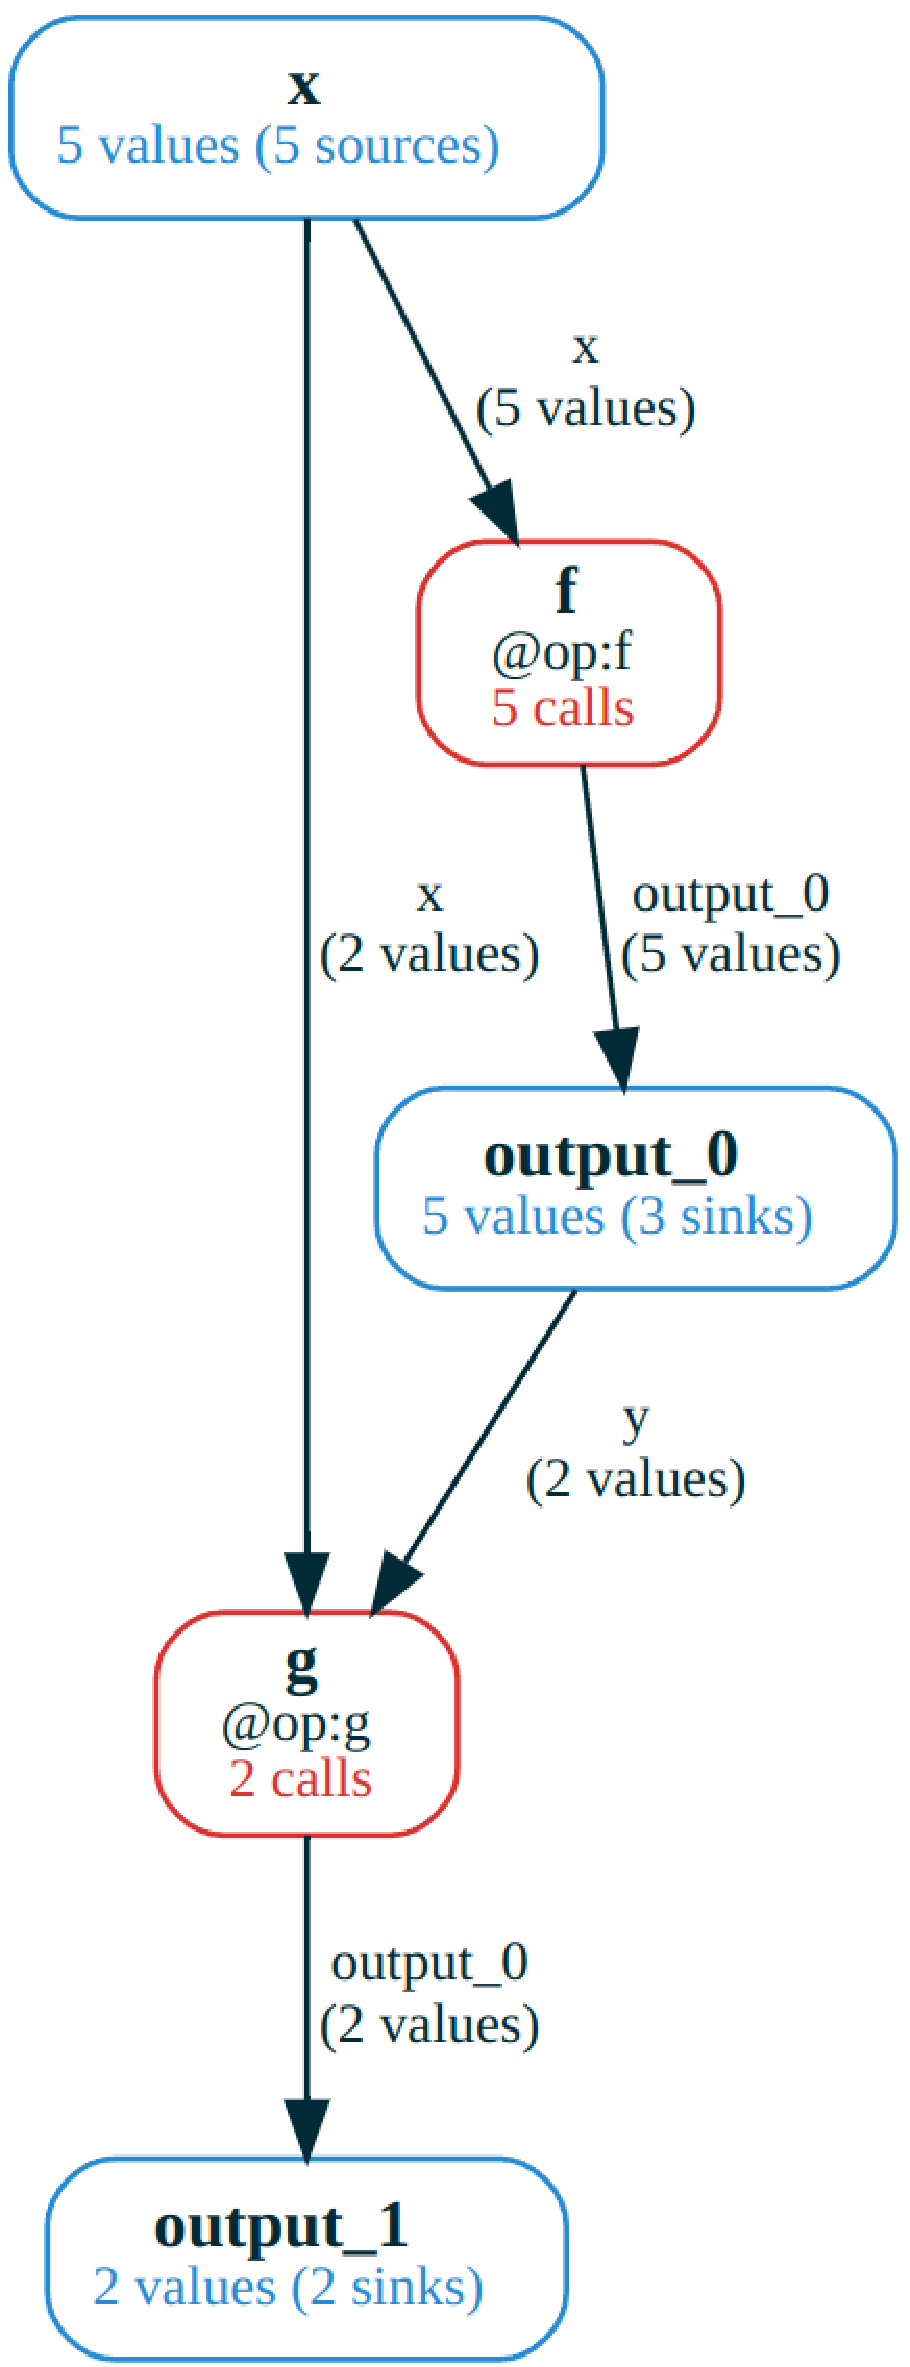
\includegraphics[width=\textwidth]{img/cf.pdf}
            \caption{A visualization of the computation frame from the previous
            two subfigures. The red nodes indicate functions, and the blue nodes
            indicate variables in the computation graph. Each edge is labeled
            with the input/output name of the adjacent function. Nodes and edges
            also show the number of \texttt{Ref}s and \texttt{Call}s they
            represent.}
            \label{fig:figure3}
        \end{subfigure}
    \end{minipage}
    \caption{Basic declarative usage of \texttt{mandala} and an example of
computation frames.}
    \label{fig:cf}
\end{figure}

In order to be able to explore and manipulate the full stored computation graph,
patterns like retracing are insufficient, because they require the complete code
producing part of the graph to be available. To complement retracing, we
introduce the \texttt{ComputationFrame} data structure, which is a high-level
declarative interface to the stored computation graph.

\subsection{Motivation and Intuition}
\label{subsection:cf-motivation-intuition}

Intuitively, a computation frame is a way to organize a collection of saved
\texttt{@op} calls into groups, where the calls in each group have an analogous
role in the computation, and the groups form a high-level computational graph of
variables (which represent groups of \texttt{Ref}s) and functions (groups of
\texttt{Call}s). The illustration in Figure \ref{fig:cf} (c) shows a
visualization of a computation frame extracted from the computations in Figure
\ref{fig:basic-usage}.

This kind of organization is useful because it reflects how the user thinks
about the computation, and allows them to tailor the exploration of the
computation graph to a particular use case, much like a database view. For
instance, sometimes it makes sense to group the outputs of several different
\texttt{@op}s into a single variable because they are treated the same way by
downstream computations.

From another point of view, computation frames are `views' of the stored
computation graph, analogous to database views. In particular, they may contain
multiple references to the same \texttt{Ref} or \texttt{Call} object from
different nodes of the graph, and do not necessarily contain all calls to a
given \texttt{@op}.

\subsection{Formal Definition}
\label{subsection:cf-definition}


A computation frame (Figure \ref{fig:cf}) consists of the following data:
\begin{itemize}
\item \textbf{Computation graph}: a directed graph $G=(V,F,E)$ where $V$ are
named variables and $F$ are named instances of \texttt{@op}-decorated functions.
The edges $E$ are labeled with the input/output names of the adjacent functions.
An example is shown in Figure \ref{fig:cf} (c);
\item \textbf{Groups of \texttt{Ref}s and \texttt{Call}s}: for each variable
$v\in V$, a set of (history IDs of) \texttt{Ref}s $R_v$, and for each function
$f\in F$ with underlying \texttt{@op} $o_f$, a set of (history IDs of) \texttt{Call}s $C_f$; 
\end{itemize}
subject to the constraint that: for every call $c\in C_f$, if there's an
input/output edge labeled $l$ connecting $f$ to some variable $v$, then if $c$
has a \texttt{Ref} $r_l$ corresponding to input/output name $l$, we have $r_l\in
R_v$. 

In other words, when we look at all calls in $f\in F$, their inputs/outputs must
be present in the variables connected to $f$ under the respective input/output
name. 

\subsection{Basic Usage}
\label{subsection:cf-basic-usage}

The main advantage of computation frames is that they allow iterative
exploration of the computation graph, and high-level grouped operations over
computations with some shared structure. For example, we can use them for:
\begin{itemize}
\item \textbf{Iteratively expanding the frame with functions that generated or
used existing variables}: this is useful for exploring the computation graph in
a particular direction, or for adding more context to a particular computation.
For example, in Figure \ref{fig:cf} (a), we start with a computation frame
containing only the calls to \texttt{f}, and then expand it to include all calls
that can be reached from the memoized calls to \texttt{f} via their
inputs/outputs, which adds the calls to \texttt{g} to the frame.
\item \textbf{Converting the frame into a dataframe}: this is useful at the end
of an exploration, when we want to get a convenient tabular representation of
the captured computation graph. The table is obtained by collecting all terminal
\texttt{Ref}s in the frame's computational graph (i.e., those that are not
inputs to any function in the frame), computing their computational history in
the frame (grouped by variable), and joining the resulting tables over the
variables. This is shown in Figure \ref{fig:cf} (right). In particular, as shown
in the example, this step may produce nulls, as the computation frame can
contain computations that only partially follow the graph.
\item \textbf{Performing high-level storage manipulations}: such as deleting all
calls captured in the frame as well as all calls that depend on them, available
using the \verb|.delete_calls()| method on the frame.
\end{itemize}

Computation frames are a powerful tool for exploring and manipulating the stored
computation graph, and we're excited to explore their full potential in future
work.

\section{Main Extra Features}
\label{section:extra-features}

\subsection{Data Structures}
\label{subsection:data-structures}

Python's native collections --- lists, dicts, sets --- can be memoized
transparently by \texttt{mandala}, using customized type annotations, e.g.
\texttt{MList[int]} inheriting from \texttt{List[int]}, \ldots. By applying this
type annotation, individual elements as well as the collection itself are
memoized as \texttt{Ref}s (with the collection merely pointing to the
\texttt{Ref}s of its elements to avoid duplication). 

\begin{wrapfigure}[18]{l}{0.45\textwidth}
    \centering
    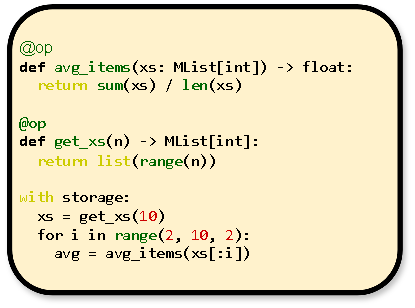
\includegraphics[width=\linewidth]{img/list.pdf}
    \caption{Illustration of native collection memoization in \texttt{mandala}.
    The custom type annotation \texttt{MList[int]} is used to memoize a list of
    integers as a list of pointers to element \texttt{Ref}s.}
    \label{fig:list}
\end{wrapfigure}

This is implemented fully on top of the core memoization machinery, using
`internal' \texttt{@op}s like e.g. \verb|__make_list__| which, given the
elements of a list as variadic inputs, generates a \texttt{ListRef} (subclass of
\texttt{Ref}) that points to the \texttt{Ref}s of the elements. In this way,
collections are naturally incorporated in the computation graph. These internal
\texttt{@op}s are applied automatically when a collection is passed as an
argument to a memoized function, or when a collection is returned from a
memoized function (Figure \ref{fig:list}).

% \subsection{Caching}
% To speed up retracing and memoization, it is necessary to avoid frequent reads
% and writes to the database backend. To this end, \texttt{mandala} implements a
% fairly standard caching system that accumulates results in memory, with the
% option to explicitly flush values to disk at once when the user decides, or
% automatically at the end of a \texttt{mandala} context. Similarly, to speed up
% retracing of existing calls, call metadata can be pre-loaded.

\subsection{Versioning}
\label{subsection:versioning}

It is crucial to have a flexible and powerful code versioning system in a data
management tool, as it allows the user to keep track of the evolution of their
computations, and to easily recover from mistakes. \texttt{mandala} provides the
option to use a versioning system with three main features:
\begin{itemize}
\item \textbf{Per-function content-addressed versioning} \citep{git,lozano2017unison}, where
the version of a function is a hash of its source code and the hashes of the
functions it calls. The storage can determine, based only on the state of the
codebase, whether a given call is up-to-date or not.
\item \textbf{Dynamic dependency tracking}, where each function call traces the
dependencies it calls. This avoids the need for static analysis of the code to
find dependencies, which can result in many false positives and negatives,
especially in a dynamic language like Python. Moreover, it provides a stronger
notion of reusability, as certain changes of the codebase may invalidate only
a part of all memoized calls to an \texttt{@op}.
\item \textbf{The flexibility to mark changes as backward-compatible or not},
which allows the user to maintain a stable interface to computations when performing routine refactoring or adding logging/debugging code.
\end{itemize}

\section{Related Work}
\label{section:related-work}

\texttt{mandala} combines ideas from several existing projects, but is unique in
the Pythonic way it makes complex memoized computations easy to query,
manipulate and version.

\textbf{Memoization.} There are several memoization solutions for Python that lack the compositional nature of \texttt{mandala}, as well as the versioning and
querying tools: the builtin \texttt{functools} module provides decorators such as \texttt{lru\_cache} for memoization; the \texttt{incpy} project \citep{guo2011using} enables automatic
persistent memoization of Python functions directly on the interpreter level; 
the \texttt{funsies} project \citep{lavigne2021funsies} is a memoization-based
distributed workflow executor that uses a similar hashing approach to keep track
of which computations have already been done; \texttt{koji} \citep{maymounkov2018koji} is a design for an incremental computation data processing framework that unifies over different resource types (files or services), and uses an analogous notion of hashing to keep track of computations.

\textbf{Computation Frames.} Computation frames are closely related to the
relational model \citep{codd1970relational}, to graph databases, and to certain
versatile in-memory data structures based on functors
$\mathcal{F}:\mathscr{C}\to \underline{\mathbf{Set}}$ where $\mathscr{C}$ is a
finite category \citep{patterson2022categorical}.

\textbf{Versioning.} The \texttt{unison} programming language
\citep{lozano2017unison} uses a content-addressed system for code storage, where
a function is identified by the hash of its syntax tree. The language shares
many other features and goals with \texttt{mandala}, such as use of serializable
values and pure functions to ensure reproducibility.

The dynamic tracing mechanism used to capture dependencies
is somewhat similar to the \texttt{@tf.function} decorator in the TensorFlow
library \citep{abadi2016tensorflow}, which traces the function calls to other
\texttt{@tf.function}-decorated functions made during execution and builds a
computation graph out of them. Unlike \texttt{@tf.function}, \texttt{mandala}'s
versioner uses content (code) hashes to automatically detect changes in
dependencies, and does not build a fine-grained model of a function's execution, but rather only tracks the set of its dependencies.

The revision history of each function in the codebase is
organized in a bare-bones \texttt{git} repository \citep{git}: it is a
content-addressed tree, where each edge tracks a diff from the content at one
endpoint to that at the other. Additional metadata indicates equivalence classes
of semantically equivalent contents. 
% Semantic versioning \citep{semver} is another popular code versioning system. 
% \texttt{mandala} is similar to semver in
% that it allows you to make backward-compatible changes to the interface and
% logic of dependencies. It is different in that versions are still labeled by
% content, instead of `non-canonical' numbers. 

\section{Limitations}
\label{sec:limitations}

\textbf{Computing deterministic content IDs of any Python object is difficult.} 
\texttt{mandala} uses the \texttt{joblib} library to serialize Python objects
into byte strings, and then hashes these strings to get the content ID. This
approach is not perfect, as it is not always possible to serialize Python
objects, and even when it is, the serialization may not be unique. For example,
two Python objects \texttt{x, y} which satisfy \texttt{x == y} may not have the
same content ID (e.g., \texttt{True} and \texttt{1}). Furthermore, hashing is
sensitive to small changes in the input, such as numerical precision in floating
point numbers. Finally, complex Python objects may contain state that is not
intrinsically part of the object's identity, such as resource utilization data
(e.g., memory addresses). This can lead to different content IDs before and 
after a round trip through the storage backend. These issues don't come up often
as long as all initial \texttt{Ref}s are created from simple Python objects:
complex objects are hashed and saved once when returned from an \texttt{@op},
and then referred to by their content ID.

\textbf{Non-breaking versioning is difficult.} The ability to mark code changes
as backward-compatible or not may lead to situations where the storage
`believes' that a call is up-to-date, but in reality it is not. For example, a
function \texttt{f} can be changed by extracting a subroutine \texttt{g} out of
it. The semantics of \texttt{f} is unchanged, so past calls are still valid,
but \texttt{g} is now an invisible (to the storage) dependency of \texttt{f}.
Care should be taken to avoid such situations until an automatic solution is
implemented.

\section{Conclusion}
\label{section:conclusion}

\texttt{mandala} is being actively developed, and has the potential to
considerably simplify the way scientific data is managed and interacted with in
Python. The author has already used it extensively to manage several multi-month
machine learning projects, and has found it to be a very powerful tool for
managing complex computations. We hope that this paper has given a good overview
of the core concepts of \texttt{mandala}, and that the reader will be interested
in exploring the library further.

\newpage

\section*{Acknowledgements}

First and foremost, I would like to thank my friend Stefan Krastanov for many
valuable conversations throughout the evolution and development of 
\texttt{mandala}. Nobody could ask for a more enthusiastic collaborator and
champion of their work. Second, I would also like to thank Nicholas Schiefer for
some helpful feedback on an earlier version of the library, as well as
suggestions and implementations for features to make it work in a distributed
setting, and for advertising \texttt{mandala} at his workplace. 

There have been far too many people over the years who have listened patiently
to me talk about this project in its earlier stages; in particular, I'm grateful
to Petar Maymounkov from Protocol Labs for inviting me to give a talk about
\texttt{mandala} at their research seminar, as well as for creating the
\texttt{escher} language, which truly changed the way I think about programming.
I'm also grateful to many friends from grad school and beyond who have listened
to me talk about this project, and who have given me valuable feedback and
encouragement. Finally, I would like to thank my reviewers at the SciPy
conference, especially Andrei Paleyes, for their helpful feedback on this paper.

% bibliography
\bibliography{scipy}
\bibliographystyle{arxiv_template}

\end{document}